\documentclass{article}

\usepackage{graphicx}
\usepackage[slovene]{babel}
\usepackage[latin2]{inputenc}
\usepackage{listings}
\usepackage{lstautogobble}
\usepackage{xcolor}
\usepackage{url}
\usepackage{hyperref}
\usepackage{booktabs} % For \toprule, \midrule and \bottomrule
\usepackage{siunitx} % Formats the units and values
\usepackage{pgfplotstable} % Generates table from .csv
\usepackage{tikz} % To generate the plot from csv
\usepackage{pgfplots}
\usepackage{float}
\usepackage[toc,page]{appendix}

\title{Uporabni�ki priro�nik za zbudim.se}
\date{21.12.2016}

\hypersetup{
	colorlinks=true
}

\pgfplotsset{
	compat=newest,
	colormap={gr}{rgb255(0cm)=(62,150,81); rgb255(1cm)=(62,150,81)}
	,colormap={bl}{rgb255(0cm)=(204,37,41); rgb255(1cm)=(204,37,41)}
} % Allows to place the legend below plot
\usepgfplotslibrary{units} % Allows to enter the units nicely

\sisetup{
	round-mode          	= places, % Rounds numbers
	round-precision     	= 3, % to 2 places
	scientific-notation 	= false,
	output-decimal-marker 	= {,}
}

\definecolor{mygreen}{rgb}{0,0.6,0}
\definecolor{mygray}{rgb}{0.5,0.5,0.5}
\definecolor{mymauve}{rgb}{0.58,0,0.82}

\lstdefinelanguage{pseudoC}{%
	language     = C,
	morekeywords = {then, Write, End, Read, Open, Initialize, Close, While, If, from, file, to},
}

\lstdefinestyle{customc}{
	belowcaptionskip=1\baselineskip,
	xleftmargin=\parindent,
	language=pseudoC,
	showstringspaces=false
}

\lstset{
	backgroundcolor=\color{gray!10!white},
	frame=L,
	basicstyle=\footnotesize\ttfamily,
	keywordstyle=\color{blue},
	commentstyle=\color{mygreen},
	stringstyle=\color{orange},
	numbers=left,
	breaklines=true,
	captionpos=b
}

\renewcommand{\lstlistingname}{Koda}

\begin{document}
	\pagenumbering{gobble}
	\maketitle
	\newpage
	\tableofcontents
	\newpage
	\pagenumbering{arabic}
	
	\section{Registracija}
	Za registracijo novega uporabnika na za�etni strani zbudim.se/login kliknite na povezavo "Registriraj se tukaj", ki je vidna tudi na sliki \ref{1}. Nato na strani, na kateri se nahajate izpolnite vse podatke (\ref{2}). Ti so email naslov, uporabni�ko ime, geslo, ki mora biti med 8 in 40 znakov dolgo in nazadnje �e ponovno vnesete geslo, kliknete da se strinjate s pogoji uporabe in kliknete na gumb registracija. Po registraciji boste na va� email naslov prejeli povezavo, katero morate obiskati �e �elite za�eti uporabljati spletno stran.
	
	\begin{figure}[H]
		\centering
		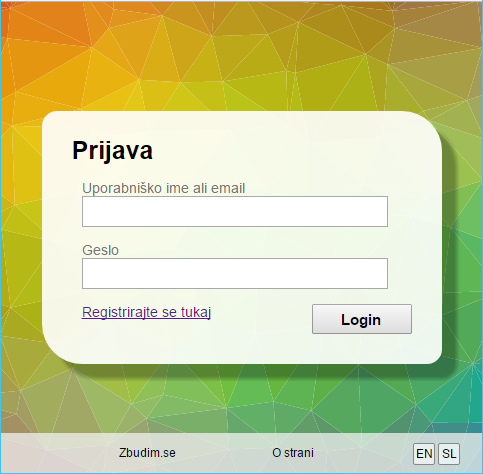
\includegraphics[width=0.5\linewidth]{1.png}
		\caption{Za�etna stran zbudim.se/login}
		\label{1}
	\end{figure}

	\begin{figure}[H]
		\centering
		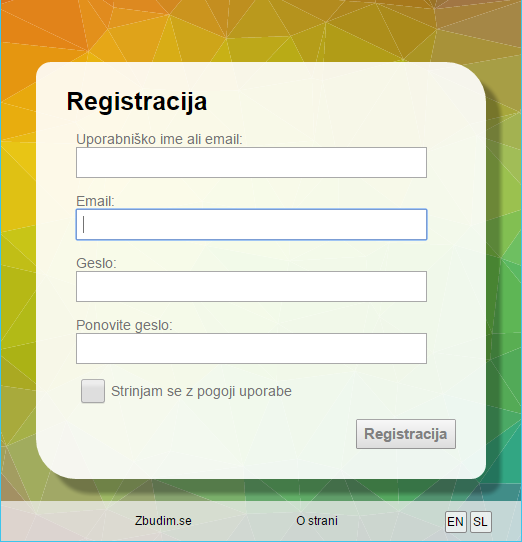
\includegraphics[width=0.5\linewidth]{2.png}
		\caption{Registracija novega uporabnika}
		\label{2}
	\end{figure}

	\section{Prijava in nastavitve}
	Za prijavo v spletno aplikacijo vnesite uporabni�ko ime ali email ter geslo na za�etni strani (slika \ref{1}). Ob prvi prijavi boste s tem pri�li do strani s nastavitvami, �e pa ste te �e izpolnili pa na glavno stran spletne aplikacije. Na strani s nastavitvami, do katerih pridete tudi s klikom na gumb nastavitve v navigaciji (slika \ref{4}), morate izpolniti osnovne podatke, kot so doma�i naslov (vklju�no s krajem), �as, ki ga potrebujete za pripravo pred odhodom od doma in prevozna sredstva, ki so vam na voljo. Po vnosu podatkov te shranite s klikom na gumb shrani. Poleg samih nastavitev je na dnu strani (slika \ref{3}) na voljo tudi vnos urnika iz uradne spletne strani fakultete na podlagi vpisne �tevilke. To storite tako da vnesete va�o vpisno �tevilko in kliknete na gumb za uvoz urnika. V nekaj minutah se bo va� urnik uvozil in se prikazal na va�i glavni strani.
	
	\begin{figure}[H]
		\centering
		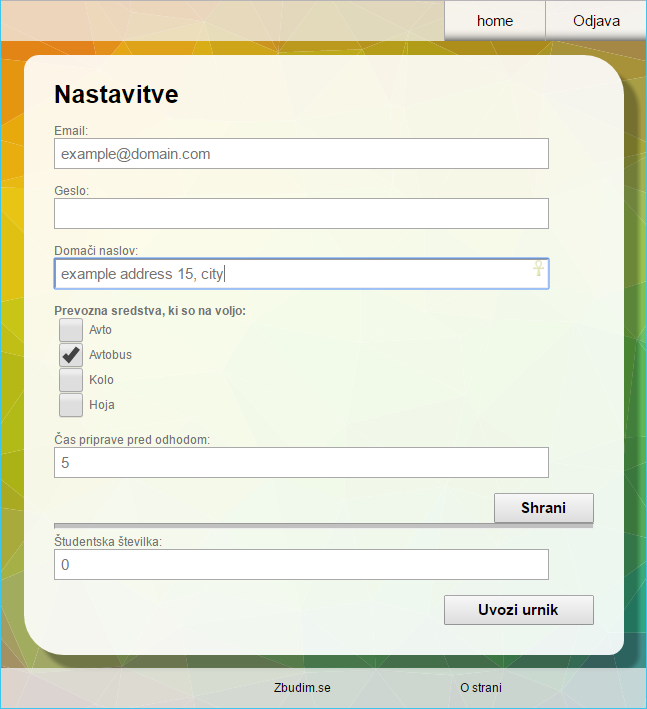
\includegraphics[width=0.5\linewidth]{3.png}
		\caption{Nastavitve spletne aplikacije}
		\label{3}
	\end{figure}

	\section{Dodajanje, odstranjevanje in menjava predavanj}
	Na glavni strani lahko dodate nova predavanja s klikom na gumb dodaj predavanje. S tem se vam bo pojavil seznam predmetov, katere lahko tudi filtrirate s iskalnim poljem. Po izbiri predmeta se bodo na desni strani pojavile ustrezna predavanja, katera lahko dodate va�emu urniku s klikom na njih. 
	
	\begin{figure}[H]
		\centering
		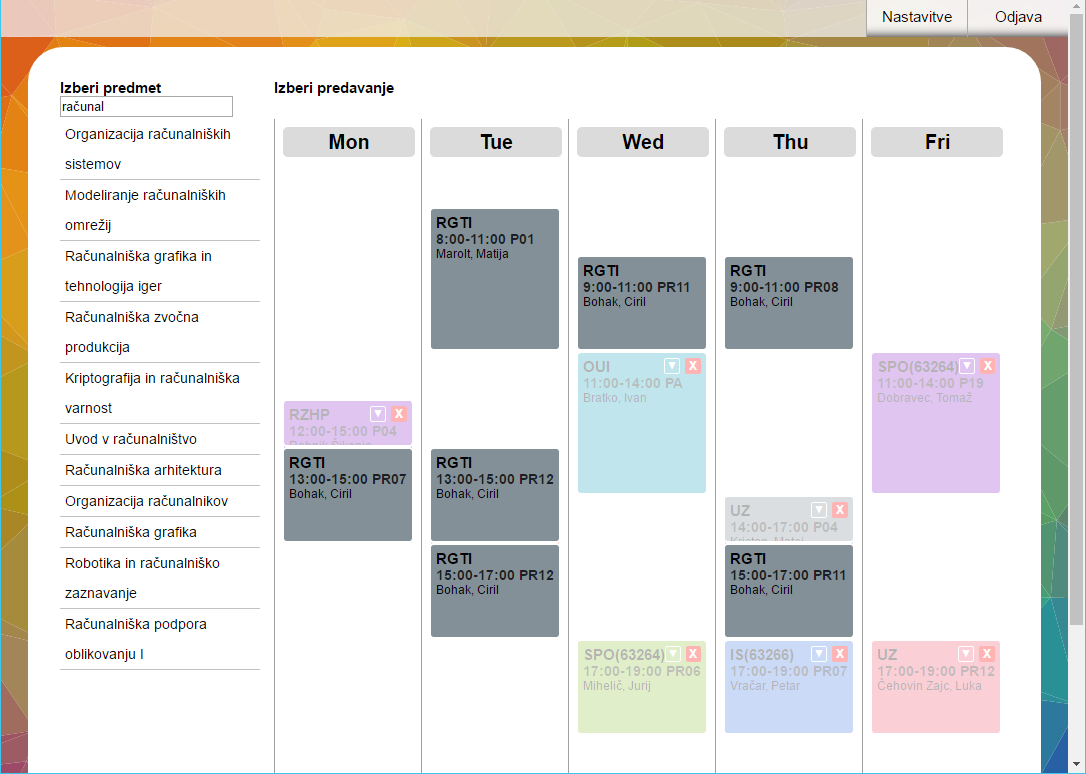
\includegraphics[width=0.5\linewidth]{4.png}
		\caption{Dodajanje predmeta}
		\label{4}
	\end{figure}

	Predmet lahko odstranite z kliko na rde� kri�ec, ki se nahaja v kotu vsakega predavanja, ali pa s klikom na ikono poleg tega in izbiro odstrani predavanje iz seznama. Poleg tega lahko v seznamu zamenjate predavanje s nekim drugim, ali pa zaprosite za zamenjavo z drugim �tudentom.
	
	\section{�as bujenja in odhoda} 
	�as odhoda od doma se izra�una s pomo�jo google directions apija, na podlagi vremena in nastavitev se dolo�i na�in prevoza, in glede na va� urnik se dolo�i ura odhoda od doma, tako da boste �e ujeli naslednje predavanje. 
	
\end{document}